\cleardoublepage
% \newpage

% % 页眉:单页印刷
% \fancyhead[L]{\zihao{-5}{\songti 重庆大学本科学生毕业论文(设计)}}
% \fancyhead[R]{\zihao{-5}{\songti 3\quad 图表、公式格式}}

% 页眉:双页印刷
\fancyhead[CE]{\zihao{-5}{\songti 重庆大学本科学生毕业论文(设计)}}
\fancyhead[CO]{\zihao{-5}{\songti 3\quad 图表、公式格式}}

\section{图表、公式格式}
\subsection{图表格式}
本章将主要介绍一些图表和公式的格式...\\

\begin{figure}[htb] 
    \center{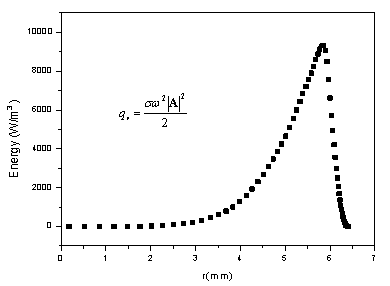
\includegraphics[width=0.9\textwidth]  {static/temp.png}} 
    \caption{内热源沿径向的分布}
\end{figure}

\begin{table}[htbp]
    \centering
    \caption{高频感应加热的基本参数}
    \small
    \begin{tabular}{c c c c}
    \toprule
    感应频率 &感应发生器功率 & 工件移动速度  &感应圈与零件间隙\\
    (KHz)&($\% \times$80Kw) &(mm/min)  &(mm)\\
    \midrule
    250 &88 &5900 &1.65\\
    
    250 &88 &5900 &1.65\\
    
    250 &88 &5900 &1.65\\
    
    250 &88 &5900 &1.65\\
    
    \bottomrule
    \end{tabular}
    \end{table}
\begin{table}[htbp]
    \centering
    \captionsetup{singlelinecheck=off}
    \caption*{续表3.1}
    \small
    \begin{tabular}{c c c c}
    \toprule
    感应频率 &感应发生器功率 & 工件移动速度  &感应圈与零件间隙\\
    (KHz)&($\% \times$80Kw) &(mm/min)  &(mm)\\
    \midrule
    250 &88 &5900 &1.65\\
    
    250 &88 &5900 &1.65\\
    \bottomrule
    \end{tabular}
    \end{table}
    \vspace{\baselineskip}
    %表格太大需要转页时,需要在续表上方注明“续表”,表头也应重复排出。
    


\subsection{公式格式}


\begin{eqnarray}
\frac{1}{\mu} \nabla^2A - j \omega \sigma A -\nabla(\frac{1}{\mu}) \times(\nabla \times A)+J_0=0
\end{eqnarray}


\subsection{本章小结}
本章介绍了……
